% 本文件是示例论文的一部分
% 论文的主文件位于上级目录的 `bachelor.tex` 或 `master.tex`

\chapter{绪论}
\section{研究背景及意义}
\subsection{研究背景}
近些年来,经济的快速增长推动了城市化发展的进程,人民生活水平日益提高,但与此同时一些“城市病”也逐渐显现出来,例如城市交通拥堵。在过去五年内,中国机动车辆的保有量在逐年增加,如\autoref{tab:vehicle-nums}所示,在2016年,中国汽车保有量超过一百万的城市数量有49个,而截至2020年汽车保有量超过一百万的城市数量已经突破了70,其中汽车保有量突破三百万的城市更是达到了13个。
不断恶化的交通拥堵情况,极大的影响了人们的日常生活,人们花费在交通通勤的时间变长也越来越常态化并且这种现象已经开始向中小城市蔓延。为此,很多城市开始研究不同的解决方案以缓解不断恶化的交通拥堵情况。对于基础建设已经趋于饱和的大城市而言,例如北京,通过出台“限号”政策来减少出行路面上的车辆数量,而对于正在发展中的中小城市而言,更多的是选择通过加快城市道路建设来加大城市交通的承载量。
虽然这些方法在一定程度上使交通拥堵得到了缓解,但是并没有从根本上解决问题。其实,交通拥堵通常是由于不同的车流为了争夺同一个“行驶资源”而造成的,在城市道路中,这一“行驶资源”通常就是车辆所处的交通路口,所以现代城市交通管理的主要方法是在道路汇合的交叉路口安装信号灯并通过简单的策略来调度通过的车流,已到达减少交通拥堵的目的。
但是随着车辆数量的不断增加,之前传统的交通信号控制策略已经难以应对现在更加复杂的交通模式。因此,如何制定出更加高效和智能的交通信号调度策略显得格外的重要。

\begin{table}[htb]
    \caption{2016-2020年汽车保有量城市数据统计(数据来源:公安部)\label{tab:vehicle-nums}}
    \begin{tabular}{lcccccc}
      \toprule
      城市汽车保有量 & 单位 & 2016年 & 2017年 & 2018年 & 2019年 & 2020年 \\
      \midrule
      \tabincell{l}{汽车保有量\\超百万城市数量} & 个 & 49 & 53 & 61 & 66 & 70 \\
      \hline
      \tabincell{l}{汽车保有量\\超两百万城市数量} & 个 & 18 & 24 & 27 & 30 & 31 \\
      \hline
      \tabincell{l}{汽车保有量\\超三百万城市数量} & 个 & 6  & 7 & 8 & 11 & 13 \\
      \hline
      \tabincell{l}{汽车保有量\\超五百万城市数量} & 个 & 1  & 1 & 1 & 2 & 3 \\
      \bottomrule
    \end{tabular}
\end{table}


随着车联网技术的发展,对于实时车辆数据的获取变得越来越容易,利用得到的车辆数据可以获得实时的交通状况,因此如何根据实时的交通状况来制定最优的调度策略一直是研究的热点。以往多数的研究是采用基于优化的方法,根据车流的状况计算出一个最优的信号灯的相位序列,但是这种方法要求车流的分布是相对稳定的,例如服从均匀分布,这一假设与现实中的车流情况相比太过理想化,所以难以部署到实际场景中。
伴随着人工智能技术的发展,一些研究者提出利用深度强化学习(Deep Reinforcement Learning,DRL)来控制信号灯,将整个交通信号灯控制建模成一个马尔可夫决策过程。对于每一次决策,输入当前的交通状况作为状态,输出一个作用在信号灯上的动作,例如变换到下一个信号相位。这种方法对于车流的分布情况没有限制,通过在大量不同的仿真车流下进行训练可以得到一个鲁棒的模型,能够应对不同的车流场景并做出最优的决策,并且这种方法在通行效率上也比基于优化的方法和传统的规则控制方法更高。

\subsection{研究意义}
\textbf{(1)传统交通信号控制方法的不足}

传统的交通信号控制方法在当下已经难以有效地减轻交通拥堵的情况。对于使用预先定义信号方式的控制方法来说,由于其信号规则是根据历史交通数据计算出来的,没有考虑实时的交通状况,所以难以有效地提高系统的通行效率。而对于使用优化方法的信号控制策略来说,由于其假设条件太过严苛,导致难以应用到实际场景中。

\textbf{(2)基于深度深度强化学习的智能交通信号调度的优点}

随着最近强化学习技术的发展,我们看到学术界对使用强化学习来改善交通信号控制的热情越来越高涨,并且也提出了很多基于深度强化学习的智能交通信号控制方法。与传统的交通信号控制方法相比,基于深度强化学习的智能交通信号调度方法有诸多优点。首先,它能够根据实时的交通状况更改交通信号,并且可以在与环境的迭代中不断地修改和提升自身调度策略的性能,从而最大程度上的提高路口的通行效率。其次,强化学习是一个无模型的方法,智能体能够在训练中进行自我学习,而不需要人为地在外部监督和操作,也不需要环境的先验知识。再者,它不需要预先定义一个能够涵盖环境中影响系统性能的所有因素的模型。

\textbf{(3)目前基于深度强化学习的智能交通信号调度工作的不足}

虽然目前已经有不少关于深度强化学习控制交通信号的研究工作,并且与传统方法相比也取得了不错的性能提升,但是任然有一些问题值得深入研究,例如公平性问题和协调通信问题。

公平性问题是指,不同车辆通过同一个路口所需的通行时间可能有很大的差别,因为信号灯可能为了提高整体通行效率而牺牲一些车辆,让这些车辆多等待一些时间,即便这些车辆可能是先进入路口的,这种做法对这些车来说是不公平的。一个好的控制策略应该在提高通行效率的同时能够保证每辆车所需的通行时间大致相同,也就是说,车辆通行时间的方差应该越小越好。但是已有的工作都是使用车辆的平均通行时间来衡量通行效率,很自然的忽略了公平性问题。

协调通信问题是指在多路口交通信号控制问题中,路口之间通过信息交互来实现多个路口的协调控制控制,从而提高整个路网的通行效率。但是已有的工作在进行信息交互时,笼统地将自身路口所有的信息传递给目标路口,会导致目标路口难以提取出有效的信息,从而增加学习的难度,甚至学习出错误的策略。


\section{国内外研究现状}
交通信号控制是城市交通管理中最有效的方法之一,为每个交叉路口提供更顺畅、更安全的交通流。从简单的自动信号控制器问世以来,交通信号控制系统一直在不断地改进,以解决造成交通信号控制障碍的因素。
\begin{figure}[htb]
    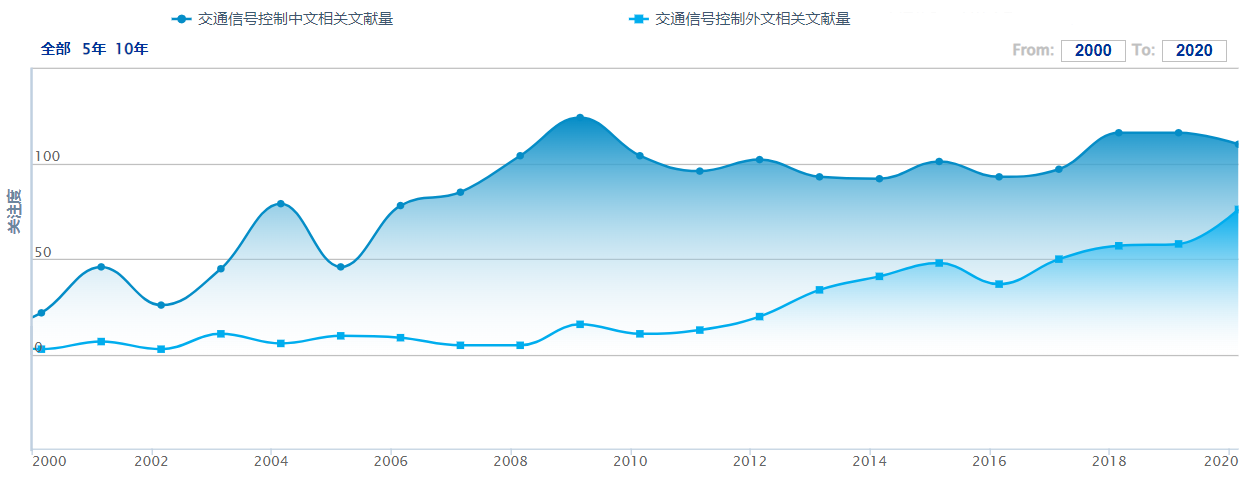
\includegraphics[width=0.9\textwidth]{fig/trend.png}
    \caption{交通信号调度国内外研究趋势(来源:中国知网研究指数统计)}
    \label{fig:trend}
\end{figure}
\autoref{fig:trend}展示了近20年来国内外关于交通信号调度的研究趋势,从中可以看出,相较于国外而言,早期国内对于交通信号调度研究的关注相对较少,但是随着近些年来国内交通拥堵情况的加重,国内学者对这方面的研究越来越感兴趣。

目前,已有的关于交通信号调度的研究主要可以分为两大类,一类是传统的交通信号控制,另一种是基于学习的智能交通信号控制。

传统交通信号控制可以细分为两类:第一类是基于预定义的信号控制(pre-defined signal control)\cite{miller1963settings},这类方法根据历史交通流量信息预先计算好交通信号的序列和周期长度,当部署到交通信号灯上就循环的在之前定义的信号序列上变换。由于没有考虑实时的交通情况,所以这类方法不能够有效地适应动态的交通变化,因此通行效率相对较低。
第二类是基于优化方法的自适应控制,这类方法通常是从优化的角度解决某些交通流模型下的交通信号控制问题,并且根据观测到的数据调整信号的序列和周期。然而,为了让问题易于求解,这些方法通常在模型上做出很强的假设\cite{baang1976optimal,silcock1997designing,haddad2010optimal}。例如,为了优化车辆通行时间,Webster在工作\inlinecite{webster1966traffic}中假设车辆的到达率是均匀的,由于这些假设条件通常太过理想化,所以难以适用于现实世界的交通流量。
此外,这类方法仅考虑当前(或)瞬时的交通状况,例如,它根据车道上时候有车辆来决定是否激活绿色信号,而不是长期的交通状况(如,队列长度)。因此,传统的交通信号控制方法缺乏对当前和长期的交通状况的同时考虑。目前,人们已经开始研究能够优化交通信号调度和计时的交通信号控制,如在适当的时候延长绿灯时间,以改善中载或重载交通的单个或多个交叉路口的交通瓶颈。

与传统交通信号控制不同的是,基于学习的智能交通信号控制不需要预先定义的规则和过多的假设条件,此外,强化学习作为一种自适应的方法,能够对当前和长期的交通状况的动态性做出反应。具体来说,这类方法直接从与环境的交互中学习,并且根据环境的反馈来完善和改进自身的控制策略,逐渐达到最优的效果。2003年,Abdulhai\cite{abdulhai2003reinforcement}首次提出了使用强化学习来自适应地改变交通信号的控制思路,为后续的研究工作指明了方向。在研究初期,智能体的状态表示都是定义成离散值的形式\cite{abdoos2013holonic,abdulhai2003reinforcement,bakker2010traffic,el2013multiagent,wiering2000multi},例如车辆的位置或者等待的车辆数量,这种做法的副作用就是离散的状态-动作值函数矩阵需要巨大的存储空间,这使得这些方法无法用于大型状态空间问题。
为了解决这个问题,Li\cite{li2016traffic}和Van der Pol\cite{van2016coordinated}使用连续状态表示的深度强化学习算法DQN(Deep Q-learning)来降低模型存贮的难度。这一类方法通过学习一个价值函数来将状态和动作对映射到奖励空间上,他们的主要区别体现在状态表示(例如,队列长度\cite{mannion2016experimental}、平均延误时间\cite{genders2016using,}和图像特征\cite{gao2017adaptive,liu2017cooperative,van2016coordinated}等)以及奖励设计(例如,平均延误时间\cite{arel2010reinforcement,van2016coordinated}、平均通行时间\cite{liu2017cooperative,van2016coordinated}和队列长度\cite{mannion2016experimental}等)。然而,这些方法都使用了相对静态的交通环境,因此与实际交通场景想去甚远。为此,Wei在\inlinecite{wei2018intellilight}工作中提出了一个新的基于强化学习的信号控制模型并首次在真实的交通数据集上进行了实验。

随着深度强化学习在单路口场景下的交通信号控制问题中取得了出色的表现,人们开始将问题拓展到多路口场景下。相对于单路口而言,多路口场景交通信号控制问题中需要考虑可拓展性问题和协调控制问题。针对可拓展性问题,Mannion在\inlinecite{mannion2016experimental}工作中使用隔离处理的方法,即对于路网下的每一个路口使用单独的交通信号控制方法。这种方法可以轻松地应对路网规模的变化,但是由于忽略了相邻路口的交通状况,所以无法实现协调控制。
关于协调控制,一种方法是通过对一个区域内的所有控制智能体进行集中优化\cite{van2016coordinated}以确保最优性。然而,随着路网规模的扩大,联合动作空间也会呈指数增长,阻碍了这种方法在大规模交通信号控制中的应用。还有一类方法试图通过去中心化的方式,即每个智能体单独控制一个路口,同时通过适当的奖励和状态设计来实现协调控制\cite{nishi2018traffic,wei2019colight}。Chen在\inlinecite{chen2020toward}中通过将智能体之间的参数进行共享实现了在仿真环境中城市级别的交通信号控制。

目前,虽然已经有不少基于强化学习的智能交通信号调度研究,但是任然有一些问题没有得到解决,有待于进一步地研究。

\section{论文主要工作}
近年来,基于深度强化学习的智能交通信号调度已经逐渐称为研究热点。然而,目前的工作对于单路口场景下的公平性调度以及多路口场景下的协调控制的研究还不够充分。本文分析了在单路口和多路口这两个不同信号调度场景下已有工作的不足,并在已有工作的基础上,分别对这两个场景下存在的问题进行了改进。本文的主要工作如下:
\begin{enumerate}
    \item 在单路口交通信号调度场景下,为了提高路口的整体通行效率,强化学习模型会偏向于优先放行交通流量大的车道,而忽略交通流量小的车道,从而导致部分车辆出现“饥饿等待”的情况。本文引入无线通信网络中Proportional Fair Scheduling(PFS)调度策略,并以此设计了一个能够在效率和公平性之间取得良好平衡的强化学习模型。通过在不同的交通负载情况下进行的实验结果表明,与传统的交通信号控制方法相比,本文提出的模型能够更大程度地提高通行效率,缓解交通路口的压力;
    与已有的基于深度强化学习的交通信号控制方法相比,我们的模型在保证系统通行效率的同时,还能够确保相对的公平性,有效地缓解的车辆“饥饿等待”的情况。
    \item 在多路口交通信号调度场景下,为了实现多路口的协调控制,目前常用的方式就是将智能体自己观测到的局部环境全部传输给相邻路口的智能体。虽然这种做法可以让智能体对全局环境有更加全面的了解,于此同时也增加了通信代价,而且还让智能体的训练难度加大。
    此外,并不是所有的信息对于其相邻的路口都是有用的,可能有些信息对其上游路口有用,有些影响其下游路口,笼统地传递所有观测信息会导致目标路口难以从这些冗余的信息中挖掘出对自身路口有效的信息,为特定路口筛选特定的信息来进行交流不仅可以减少通信代价,而且可以让学习的效率提高。
    本文在已有工作的基础上提出了一种新的针对道路网的建图方式,在这种方式下,目标路口在聚合邻近路口交通信息时可以自动剔除与自身无关的交通流量信息,从而快速的实现信息聚合。通过在合成交通数据和真实交通数据上进行实验,结果表明这种新的建图方式可以有效提高系统的通行效率以及学习模型的收敛速度。
\end{enumerate}
\section{论文组织结构}
论文总共分为五章,其组织结构如\autoref{fig:paper-struct}所示,各章节的安排如下:

\begin{figure}[htb]
    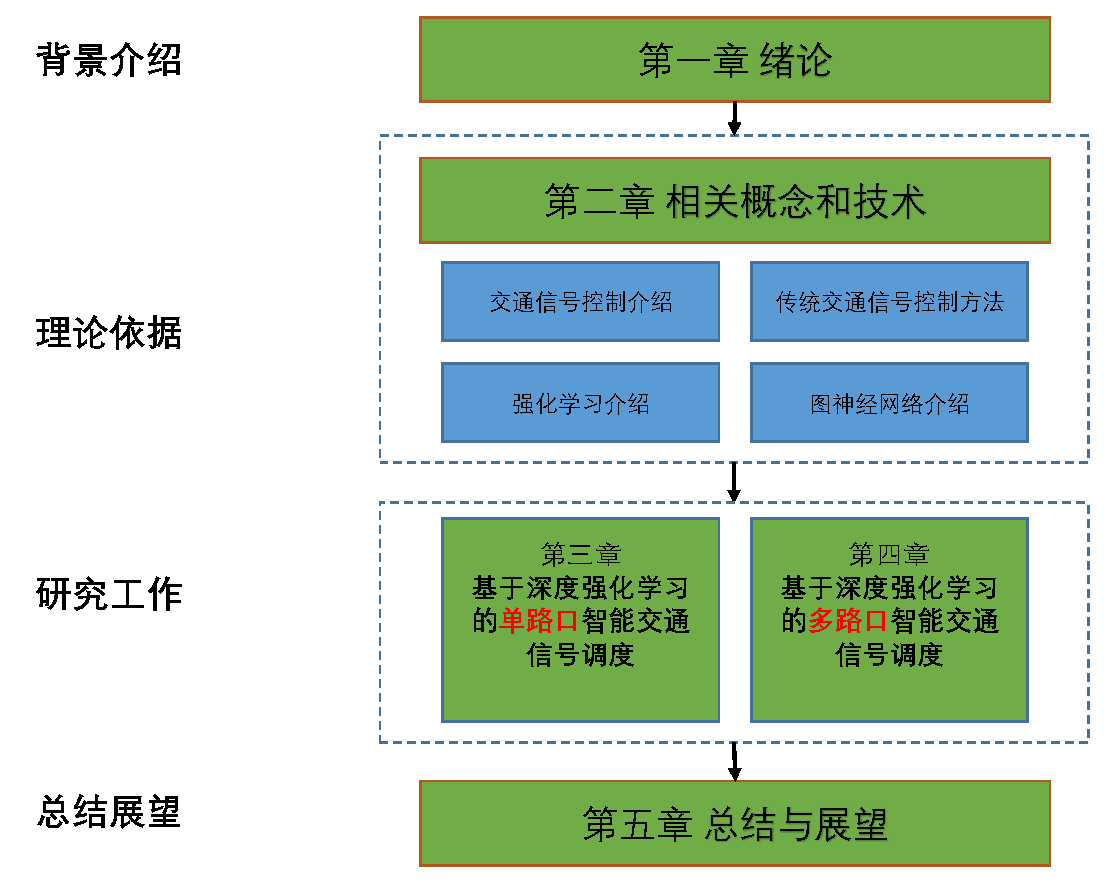
\includegraphics[width=0.8\textwidth]{fig/paper-struct.pdf}
    \caption{论文组织结构}
    \label{fig:paper-struct}
\end{figure}
第一章:绪论。结合交通拥堵情况恶化的严峻趋势,提出了高效的交通信号调度方法的重要性,并进一步给出了使用强化学习解决交通信号调度问题的重要意义。再次基础上,总结了基于强化学习的智能交通信号调度的研究现状,介绍了本文的主要研究工作以及具体的研究内容。

第二章:相关概念和技术。介绍了传统的交通信号控制方法以及基于深度强化学习的智能交通信号调度的技术背景,包括深度强化学习以及图神经网络。

第三章:基于深度强化学习的单路口智能交通信号调度。针对为了提高系统通行效率而忽视小交通流量导致的车辆“饥饿等待”问题,引用无线网络中的Proportional Fair调度方法,提出了一种新的在提高通行效率的同时保证整体相对公平的基于强化学习的智能交通信号调度方法,最后给出了仿真实验结果并与已有的方法进行了对比分析。

第四章:基于深度强化学习的多路口智能交通信号调度。针对多路口协调控制中出现的信息冗余问题,提出了一种基于新的路网建图方式的多路口交通信号调度模型来自动剔除对目标路口无关的交通流量,从而降低提取有效信息的难度,最后在仿真环境中分别就合成数据和真实数据进行了实验,并对比分析了提出的模型的性能。

第五章:总结与展望。总结了本文在基于深度强化学习的智能交通信号调度方面所作的工作,并提出了下一步智能交通信号调度的研究方向。

\section{本章小结}
本章交通信号控制的背景入手,分析的智能交通信号调度的重要性,给出了研究基于深度强化学习的智能交通信号调度的研究意义。并在此基础上,总结了基于深度强化学习的智能交通信号调度的研究现状,给出了本文的主要研究工作。最后,介绍了论文的结构安排。